%% Timelines page: how are the instances of one well distributed in time?
%%
%% Every figure quoted here is a macro of figures/timelines/numbers.tex; the
%% charts are figures/timelines/*.tikz, each reading a CSV table beside it, and
%% the tabulars are tables/timelines/*.tex. The numbers, the CSV tables and the
%% two crops of the viewer are written by scripts/timelines.py (see README.md).
%% Three frames: the overlaps, what a joined history is labeled as, and the
%% histories whose labels do not add up; the appendix shows those histories.

% Written by scripts/timelines.py from the catalogue of 3W; do not edit by hand.
\newcommand{\tlWells}{40}
\newcommand{\tlWellsOverlapping}{17}
\newcommand{\tlWellsApart}{23}
\newcommand{\tlInstances}{1,119}
\newcommand{\tlInstancesOverlapping}{986}
\newcommand{\tlPairs}{912}
\newcommand{\tlPairsAcrossFolders}{7}
\newcommand{\tlCollisions}{0}
\newcommand{\tlStackedAfterJoin}{0}
\newcommand{\tlRows}{32,872,250}
\newcommand{\tlRowsDistinct}{29,709,635}
\newcommand{\tlRowsTwice}{3,162,615}
\newcommand{\tlRowsTwiceShare}{9.6}
\newcommand{\tlJoinedBars}{208}
\newcommand{\tlUnlabeledBefore}{12.3}
\newcommand{\tlUnlabeledBeforeHours}{1,119}
\newcommand{\tlFilesWithUnlabeledHour}{1,119}
\newcommand{\tlUnlabeledAfter}{2.9}
\newcommand{\tlUnlabeledAfterHours}{240}
\newcommand{\tlGaps}{1,106}
\newcommand{\tlHeadsIntoNormal}{177}
\newcommand{\tlReturnsWithinFiles}{0}
\newcommand{\tlReturns}{13}
\newcommand{\tlReturnsWells}{7}
\newcommand{\tlReturnsAcrossFolders}{4}
\newcommand{\tlGapHeadCount}{208}
\newcommand{\tlGapHeadShare}{86.5}
\newcommand{\tlGapHeadMedian}{1\thinspace{}h}
\newcommand{\tlGapHeadMax}{1\thinspace{}h}
\newcommand{\tlGapSeamCount}{882}
\newcommand{\tlGapSeamShare}{11.5}
\newcommand{\tlGapSeamMedian}{76\thinspace{}s}
\newcommand{\tlGapSeamMax}{56\thinspace{}min}
\newcommand{\tlGapChangeCount}{16}
\newcommand{\tlGapChangeShare}{2.0}
\newcommand{\tlGapChangeMedian}{6\thinspace{}min}
\newcommand{\tlGapChangeMax}{1\thinspace{}h}
\newcommand{\tlServiceFiles}{57}
\newcommand{\tlServiceOnlyNormal}{43}
\newcommand{\tlServiceNormalShare}{84}
\newcommand{\tlServiceSteadyShare}{0.7}
\newcommand{\tlScalingFiles}{36}
\newcommand{\tlScalingNeverSteady}{31}


\newcommand{\tlquestion}{\wspage{Timelines page} \raisebox{.75pt}{$\blacktriangleright$}~How are the instances of one well distributed in time?}

% ---------------------------------------------------------------------------
\begin{frame}{Overlapping samples}
  \framesubtitle{\tlquestion}
  \begin{columns}[T]
    \begin{column}{0.47\textwidth}
      {\scriptsize\color{ws3wbrown} \tlWellsOverlapping (42.5\%) wells have overlaps, 
      totalling \tlInstancesOverlapping (88.11\%) instances\par}
      \vskip 1mm
      % The instances of the wells whose instances overlap: each well's instances in
% grey, the overlapping ones in blue over them; the tag sits at the end of the
% grey bar, which a stack would not draw for the wells whose instances all
% overlap. The table is written by scripts/timelines.py. The blue is the
% Availability chart's (the viewer's "live", light theme), so that the deck's
% bar charts share one.
\definecolor{tloverlap}{HTML}{4F6D8F}
\begin{tikzpicture}
  \begin{axis}[
      xbar, bar shift=0pt, bar width=1.8mm, scale only axis, width=48mm, height=37mm,
      y dir=reverse, ytick=data, yticklabels from table={figures/timelines/overlaps.csv}{label},
      enlarge y limits={abs=1.6mm}, xmin=0, xmax=380, xtick={0,100,200,300},
      axis x line*=bottom, axis y line*=left, y axis line style={draw=none},
      tick label style={font=\tiny, text=ws3wbrown}, ytick style={draw=none},
      legend style={font=\tiny, draw=none, fill=none, at={(1,0.02)}, anchor=south east},
      legend cell align=left, area legend, reverse legend,
    ]
    \addplot [fill=ws3wgrey!70, draw=none,
              nodes near coords, point meta=explicit symbolic,
              every node near coord/.style={font=\tiny, text=ws3wnavy, anchor=west}]
      table [x=instances, y expr=\coordindex, meta=tag] {figures/timelines/overlaps.csv};
    \addplot [fill=tloverlap, draw=none]
      table [x=overlapping, y expr=\coordindex] {figures/timelines/overlaps.csv};
    \legend{instances, overlapping another}
  \end{axis}
\end{tikzpicture}

    \end{column}
    \begin{column}{0.49\textwidth}
      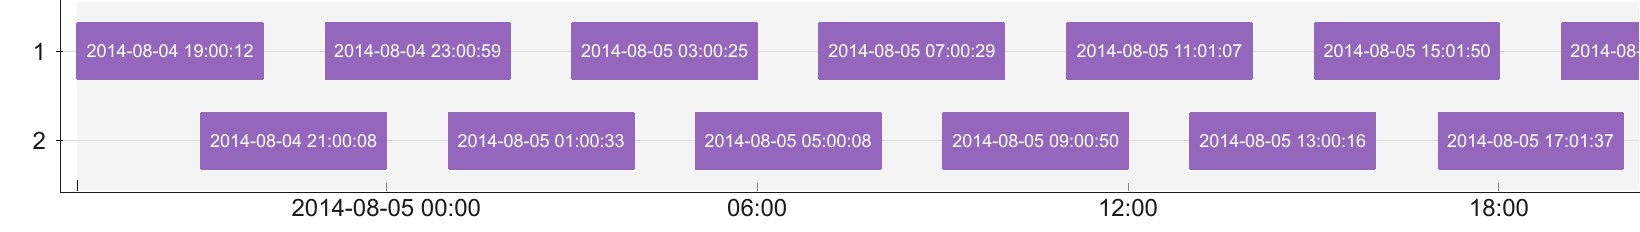
\includegraphics[width=\linewidth]{figures/timelines/well4_overlaps.png}
      {\scriptsize\color{ws3wbrown} Instances overlapping in WELL-00004.\par}
      \vskip 1.5mm
      \footnotesize
      Worries:
      \begin{itemize}
        \item Overlapping samples may land in \textbf{train and test}, causing leakage.
        \item Duplicated stretches pull \textbf{clusters} tighter, inflating scores.
      \end{itemize}
      Thankfully, 3W 2.0.0 has no label collisions, making joins principled and avoiding leakage.
    \end{column}
  \end{columns}
  \centering
  \vfill
  \alert{Clustering must still be carefully calculated!}
  \vfill
\end{frame}

% ---------------------------------------------------------------------------
\begin{frame}{What a joined history is labeled as}
  \framesubtitle{\tlquestion}
  \begin{columns}[T]
    \begin{column}{0.47\textwidth}
      \wsstat{\tlUnlabeledBefore\,\% \raisebox{1.5pt}{$\triangleright$} \tlUnlabeledAfter\,\%}{
        of unlabels after join
      }
      \footnotesize
      After the join, most unlabeled stretches appear trivial and might be recoverable.
      \vskip 2mm
      \setlength{\tabcolsep}{2pt}
      \centering
      % What a joined history leaves unlabeled, by where the stretch sits; the
% figures are macros of figures/timelines/numbers.tex.
\begin{tabular*}{\linewidth}{@{\extracolsep{\fill}} p{25mm} c p{18mm} c}
  \toprule
  \br{25mm}{Unlabeled stretch\\ position} & \textit{n} & Duration & Share \\
  \midrule
  head of a recording & \tlGapHeadCount & 1\,h each & \tlGapHeadShare\,\% \\
  \midrule
  \br{25mm}{seam between\\ equal labels} & \tlGapSeamCount & \br{16mm}{median \tlGapSeamMedian,\\ max \tlGapSeamMax} & \tlGapSeamShare\,\% \\
  \midrule
  \br{25mm}{between two labels\\ \hyperlink{changes}{\beamergotobutton{Appendix}}} & \tlGapChangeCount & \br{18mm}{median \tlGapChangeMedian,\\ max \tlGapChangeMax} & \tlGapChangeShare\,\% \\
  \bottomrule
\end{tabular*}

    \end{column}
    \begin{column}{0.5\textwidth}
      {\scriptsize\color{ws3wbrown} Each fault folder's recorded time, by label, its files apart and joined\par}
      \vskip 1mm
      % Each fault folder's recorded time by label, as a pair of bars: its files
% apart (the upper bar) and joined (the lower), every instant of a joined
% history counted once. pgfplots stacks every plot of an axis onto the one
% before, so the two stacks are drawn instead as overlaid bars from zero to
% each cumulative share, the longest first: the whole bar (its unlabeled end),
% then up to the end of steady, of transient and of normal. The tables are
% written by scripts/timelines.py.
\begin{tikzpicture}
  \begin{axis}[
      xbar, bar shift=0pt, bar width=1.5mm, scale only axis, width=30mm, height=50mm,
      y dir=reverse, ytick={0,...,9},
      yticklabels from table={figures/timelines/labels-pre-join.csv}{name},
      enlarge y limits={abs=2.4mm}, xmin=0, xmax=100, xtick={0,50,100},
      xticklabel={\pgfmathprintnumber{\tick}\,\%},
      axis x line*=bottom, axis y line*=left, y axis line style={draw=none},
      tick label style={font=\tiny, text=ws3wbrown}, ytick style={draw=none},
      legend style={font=\tiny, draw=none, fill=none, at={(0.5,1.02)}, anchor=south,
                    legend columns=4, /tikz/every even column/.append style={column sep=2mm}},
      area legend, reverse legend, clip=false,
      normal/.style={fill=ws3wblue!25, draw=none},
      transient/.style={fill=ws3wblue!55, draw=none},
      steady/.style={fill=ws3wblue, draw=none},
      unlabeled/.style={fill=ws3wgrey!45, draw=none,
                        postaction={pattern=north east lines, pattern color=ws3wbrown!60}},
    ]
    % The files apart.
    \addplot [unlabeled] table [x expr=\thisrow{normal}+\thisrow{transient}+\thisrow{steady}+\thisrow{unknown},
                                y expr=\coordindex-0.2] {figures/timelines/labels-pre-join.csv};
    \addplot [steady] table [x expr=\thisrow{normal}+\thisrow{transient}+\thisrow{steady},
                             y expr=\coordindex-0.2] {figures/timelines/labels-pre-join.csv};
    \addplot [transient] table [x expr=\thisrow{normal}+\thisrow{transient},
                                y expr=\coordindex-0.2] {figures/timelines/labels-pre-join.csv};
    \addplot [normal] table [x=normal, y expr=\coordindex-0.2] {figures/timelines/labels-pre-join.csv};
    \legend{unlabeled, steady, transient, normal}
    % The files joined.
    \addplot [unlabeled, forget plot] table [x expr=\thisrow{normal}+\thisrow{transient}+\thisrow{steady}+\thisrow{unknown},
                                             y expr=\coordindex+0.2] {figures/timelines/labels-post-join.csv};
    \addplot [steady, forget plot] table [x expr=\thisrow{normal}+\thisrow{transient}+\thisrow{steady},
                                          y expr=\coordindex+0.2] {figures/timelines/labels-post-join.csv};
    \addplot [transient, forget plot] table [x expr=\thisrow{normal}+\thisrow{transient},
                                             y expr=\coordindex+0.2] {figures/timelines/labels-post-join.csv};
    \addplot [normal, forget plot] table [x=normal, y expr=\coordindex+0.2] {figures/timelines/labels-post-join.csv};
    % Which bar is which, beside the first pair.
    \node [anchor=west, font=\tiny, text=ws3wbrown, inner sep=1pt] at (axis cs:100,-0.2) {apart};
    \node [anchor=west, font=\tiny, text=ws3wbrown, inner sep=1pt] at (axis cs:100,0.2) {joined};
    \node [anchor=west, font=\tiny, text=ws3worange, align=left] at (axis cs:101,9)
      {\textbf{\tlServiceOnlyNormal{} of \tlServiceFiles{} files}\\never leave normal};
    \node [anchor=west, font=\tiny, text=ws3wnavy, align=left] at (axis cs:101,7)
      {\tlScalingNeverSteady{} of \tlScalingFiles{} files\\never reach steady};
  \end{axis}
\end{tikzpicture}

    \end{column}
  \end{columns}
\end{frame}

% ---------------------------------------------------------------------------
\begin{frame}{Histories whose labels do not add up}
  \framesubtitle{\tlquestion}
  \begin{columns}[T]
    \begin{column}{0.52\textwidth}
      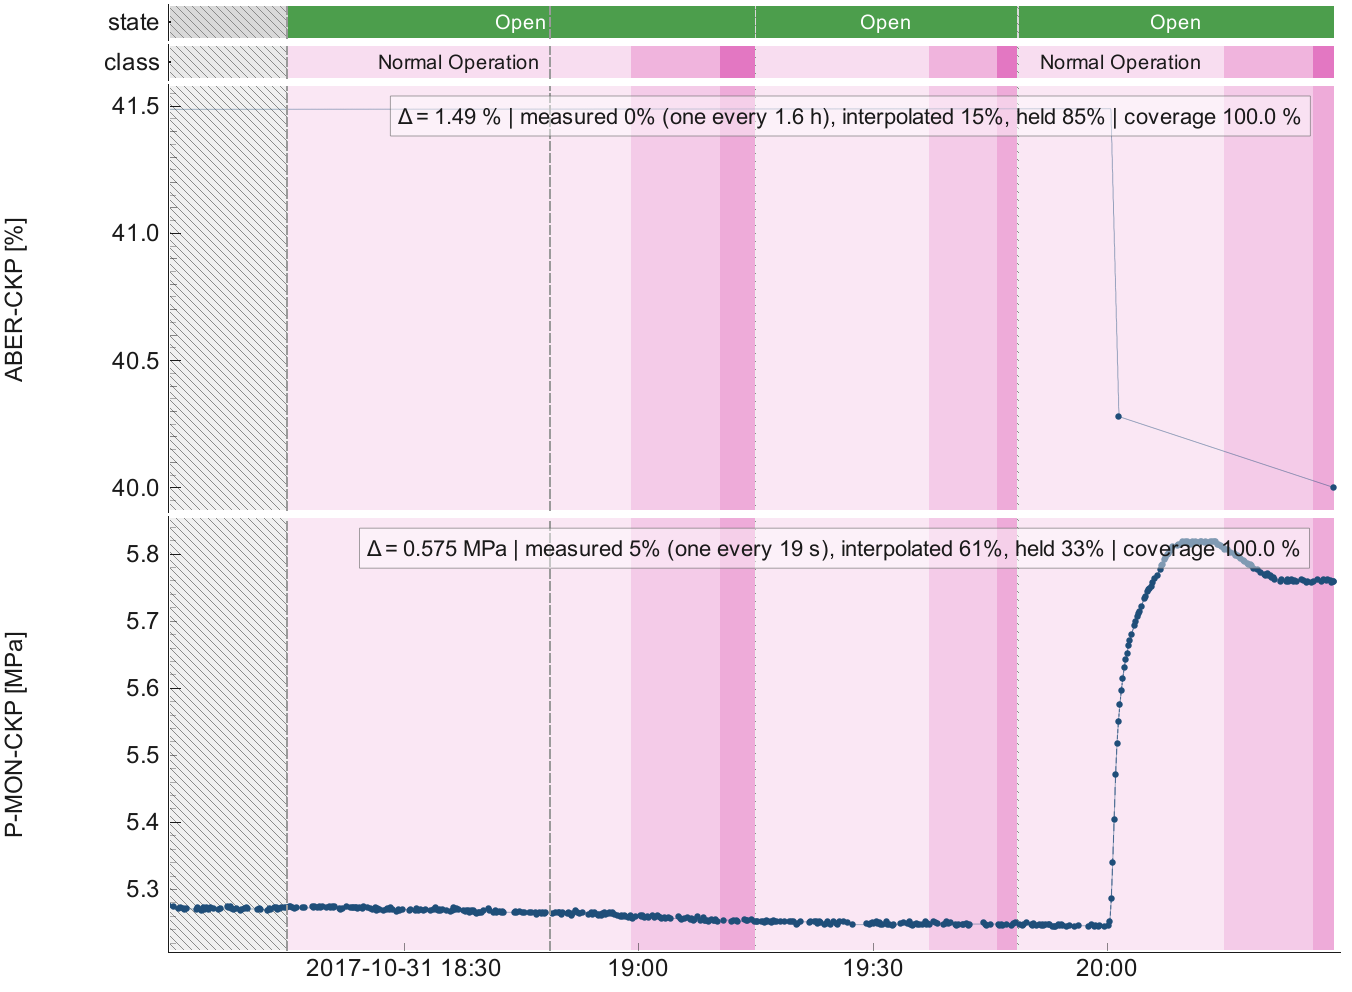
\includegraphics[width=\linewidth]{figures/timelines/well4_restrictions.png}
      {\scriptsize\color{ws3wbrown} WELL-00004's joined Quick Restriction in PCK instances.}
    \end{column}
    \begin{column}{0.45\textwidth}
      \footnotesize
      % The cases are figures/timelines/returns.csv, one row per return to normal.
      \begin{itemize}
        \item Joined histories go back to normal \textbf{\tlReturns{} times} in
          \tlReturnsWells{} wells, \textbf{every time at a file boundary}.
        \item \textbf{WELL-00004}, left: three quick restrictions in 75\,min, each back to
          normal 5 to 15\,s after its steady state.
        \item \textbf{WELL-00006}: Abrupt Increase of BSW, steady, then normal 30\,min later in
          a Scaling in PCK file.
        \item The others: Flow Instability (WELL-00001, 00004), Rapid Productivity Loss (00016,
          00020), Scaling in PCK (00024), Hydrate in Service Line (00042).
          \hyperlink{changes}{\beamergotobutton{Appendix}}
      \end{itemize}
    \end{column}
  \end{columns}
\end{frame}
